%%%%%%%%%%%%%%%%%
% Methodology %
%%%%%%%%%%%%%%%%%

This study builds on a rich body of road and graph network research by analyzing the similarities between different road networks.

\begin{figure}[h]
\centering
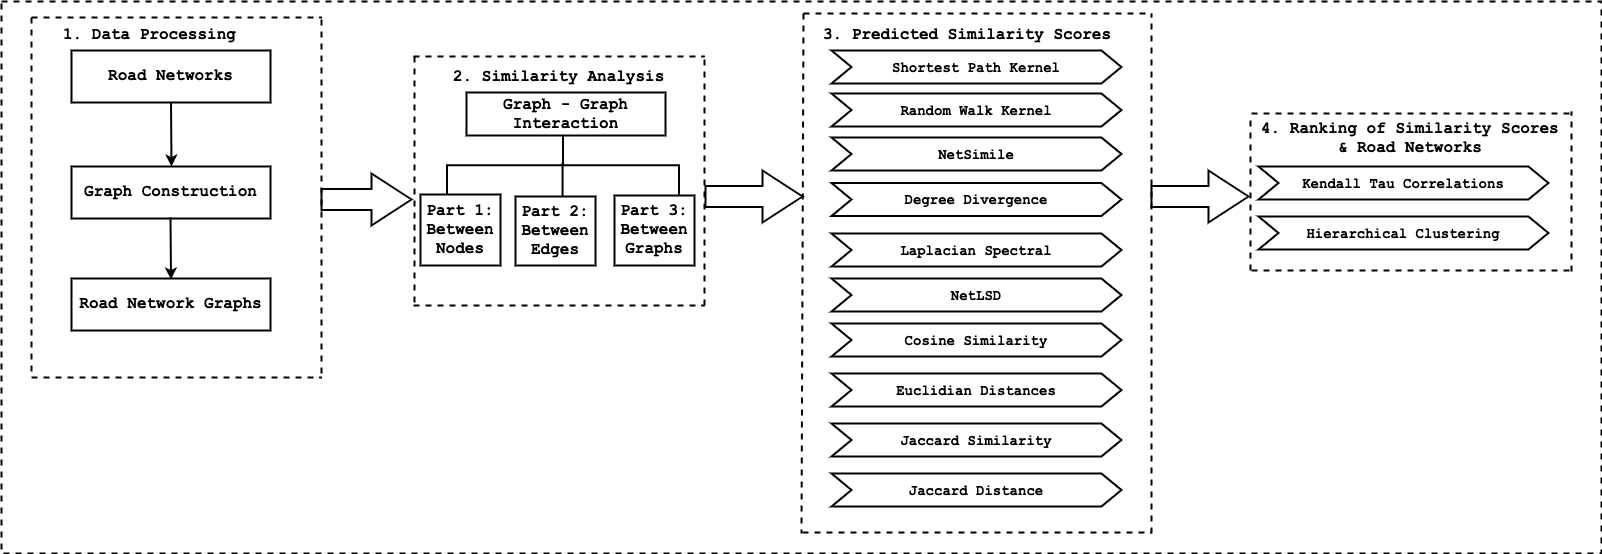
\includegraphics[width=1.25\textwidth,center]{picture/flows.png}
\caption[Miniaturtrichter]{Methodology flow}
\label{fig:flows}
\end{figure}

\section{Software}
\subsection{Python}
The coding implementation will be fully done in the Python3 programming language. In addition, open source libraries based on python will be extensively used for this thesis project.

\subsection{OSMnx}
OSMnx is a free, open-source, Python-based toolkit to automatically download spatial data (including municipal boundaries and streets) from OpenStreetMap (OSM) and construct graph-theoretic objects for network analysis (Boeing, 2017). It differentiates between walkable and drivable routes based on individual elements’ metadata that describe how the route may be used. Thus the walkable network may contain surface streets, paths through parks, pedestrian flyovers, passageways between buildings, and other walkable paths. The drivable network may contain surface streets, grade-separated freeways, and other drivable routes. OSMnx is built on top of Python's NetworkX, matplotlib, and geopandas libraries for rich network analytic capabilities, beautiful and simple visualizations, and fast spatial queries with R-tree indexing.

\subsection{Scikit-learn}
Scikit-learn is a free and open source machine learning library that can perform both supervised and unsupervised learning. It also includes a variety of tools for model fitting, data preprocessing, model selection and evaluation, and a variety of other utilities.

\subsection{Scipy}
SciPy is a free and open-source Python library for scientific and technical computing. [Pauli Virtanen; Ralf Gommers; Travis E. Oliphant; et al. (3 February 2020). "SciPy 1.0: fundamental algorithms for scientific computing in Python" (PDF). Nature Methods. 17 (3): 261–272. doi:10.1038/S41592-019-0686-2. ISSN 1548-7091. PMC 7056644. PMID 32015543. Wikidata Q84573952.] SciPy includes modules for optimization, linear algebra, integration, interpolation, special functions, FFT, signal and image processing, ODE solvers, and other tasks common in science and engineering.

\section{Data}
\begin{figure}[h!]
\centering
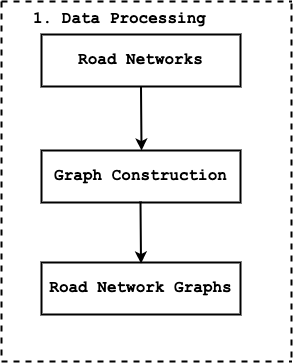
\includegraphics[width=0.25\textwidth,center]{picture/flow1.png}
\caption[Miniaturtrichter]{Data processing flow}
\label{fig:flows}
\end{figure}

The similarity analysis will be performed on 21 major cities worldwide, following Louf and Barthelemy's (2014) sampling strategy of selecting cities based on a balance of high population, regional significance, and some stratification to ensure geographical diversity within regions. The 21 sampled cities span across Africa, Asia, Australia, Europe, Middle East, North America and South America. As a result, all samples represent a diverse range of historical, cultural, developmental, and design paradigms. Of course, there is no universally accepted definition of "city" or its spatial jurisdiction throughout the world, as these differ between countries for historical and political reasons. The aim is for consistency, by trying to use each study site’s closest approximation of a “municipality” for the city limits. Once these study sites are defined,  the OSMnx software is used to download the data and road network type for each city from OpenStreetMap. Due to its high-quality worldwide coverage, OpenStreetMap (OSM) is a collaborative online mapping platform commonly used by researchers. OpensStreetMap also provides extensive, user-contributed, open data on transport networks. OpenStreetMap’s raw data contain many interstitial nodes in the middle of street segments (forming an expansion graph) to allow streets to curve through space via a series of straight-line approximations. OSMnx automatically simplifies the topology for each graph to retain nodes only at intersections and dead-ends, while retaining for each edge their true spatial geometry. This provides accurate intersection counts and edge length measures for comparison between  networks with planar and nonplanar representations.

\section{Selected Cities}
As previously stated, this study selected 21 urban road networks from around the world, which are listed in Table 3.1, along with their characteristic urban form and Node and Edge size count, to determine whether road network types in different regions share any similarities. As discussed in Chapter 2, road network data sets can be classified into five basic pattern types: tree-like, grid, cul-de-sac, linear, and radial. Despite the fact that the number of 21 data sets appears to be small, this study believes that these data sets demonstrate the dependability of the study objectives and results for the following reasons. First, despite the fact that the appearance of the city varies greatly, the main pattern differences in the urban road network can be found in the shape of intersections and the density of the road network. The only thing that needs to be determined in a classification study are the characteristics of the reference network; it is not necessary to identify all of the networks one by one. Over Reliance on large-scale statistical data may make accurate identification of road network features impossible, as some features may become submerged in the massive statistical values. [Classification of Urban Street Networks Based on Tree-Like Network Features Baorui Han 1 , Dazhi Sun 2,*, Xiaomei Yu 1, Wanlu Song 1 and Lisha Ding 1] Furthermore, approximately 40 road network samples were chosen for this study on a preliminary basis. To clearly express the road network boundary and data distribution, city samples with similar patterns and parameters were removed.
Furthermore, each sample area was limited to two square kilometers for ease of comparison. (one kilometer by one kilometer)


% Please add the following required packages to your document preamble:
% \usepackage{lscape}
\begin{landscape}
\begin{table}[]
\begin{tabular}{|l|l|l|l|l|l|}
\hline
\multicolumn{1}{|c|}{\textbf{City}} &
  \multicolumn{1}{c|}{\textbf{Country}} &
  \multicolumn{1}{c|}{\textbf{Road Network Pattern (Drive)}} &
  \multicolumn{1}{c|}{\textbf{Continent}} &
  \multicolumn{1}{c|}{\textbf{Nodes}} &
  \multicolumn{1}{c|}{\textbf{Edges}} \\ \hline
Jerusalem                       & Israel      & Cul-de-sac                & Asia          & 387  & 671  \\ \hline
Amsterdam                       & Netherlands & Cul-de-Sac                & Europe        & 547  & 1049 \\ \hline
Nairobi                         & Kenya       & Radial                    & Africa        & 410  & 793  \\ \hline
District of Columbia            & USA         & Grid                      & North America & 461  & 1167 \\ \hline
Berlin                          & Germany     & Grid                      & Europe        & 270  & 665  \\ \hline
Helsinki                        & Finland     & Grid                      & Europe        & 417  & 913  \\ \hline
Toronto                         & Canada      & Grid                      & North America & 325  & 827  \\ \hline
St, Petersburg, Florida         & USA         & Grid                      & North America & 353  & 1069 \\ \hline
Belgrano, Buenos Aires          & Argentina   & Grid                      & South America & 369  & 697  \\ \hline
Roda Island, Cairo              & Egypt       & Radial                    & Africa        & 1036 & 2520 \\ \hline
Jumeirah Islands, Dubai         & UAE         & Linear                    & Asia          & 93   & 198  \\ \hline
Jakarta                         & Indonesia   & Linear                    & Asia          & 242  & 403  \\ \hline
Sydney                          & Australia   & Linear                    & Australia     & 66   & 121  \\ \hline
Connaught Place, New Delhi      & India       & Radial                    & Asia          & 391  & 853  \\ \hline
Champs-Elysees, Paris           & France      & Radial                    & Europe        & 443  & 886  \\ \hline
Athens                          & Greece      & Shifted Grid              & Europe        & 780  & 1405 \\ \hline
Palmanova,Friuli-Venezia Giulia & Italy       & Radial                    & Europe        & 172  & 405  \\ \hline
Surulere, Lagos                 & Nigeria     & Radial                    & Africa        & 280  & 629  \\ \hline
Ejecutivo, Mexico City          & Mexico      & Shifted Grid              & South America & 530  & 1260 \\ \hline
Copenhagen                      & Denmark     & Shifted Grid, Rectangular & Europe        & 421  & 875  \\ \hline
Mumbai                          & India       & Tree                      & Asia          & 363  & 826  \\ \hline
City of Westminster, London     & UK          & Tree                      & Europe        & 607  & 1346 \\ \hline
\end{tabular}
\caption{}
\label{tab:Selected Cities}
\end{table}
\end{landscape}

\begin{figure}[h!]
\centering
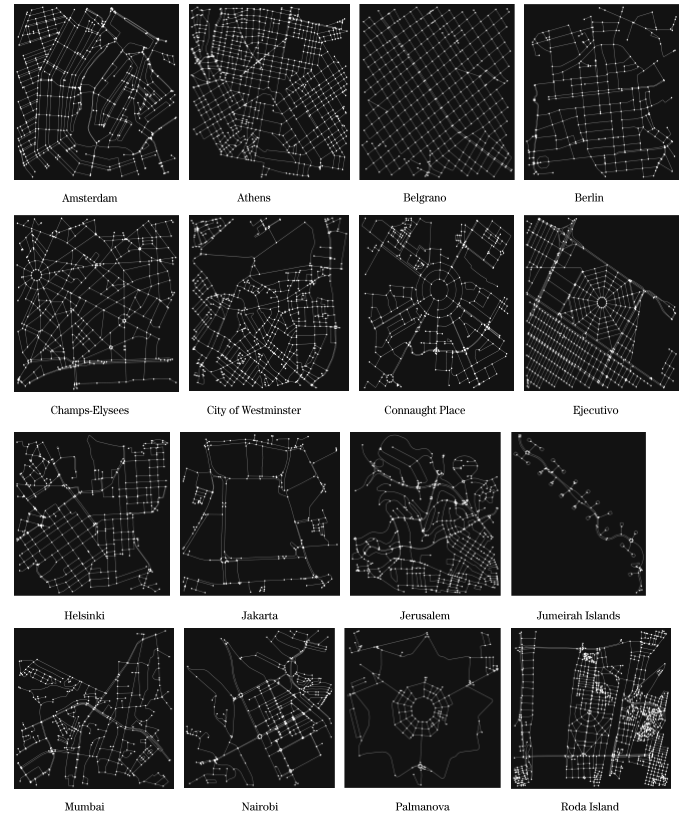
\includegraphics[width=1.0\textwidth,center]{picture/Graphs1.png}
\end{figure}

\begin{figure}[h!]
\centering
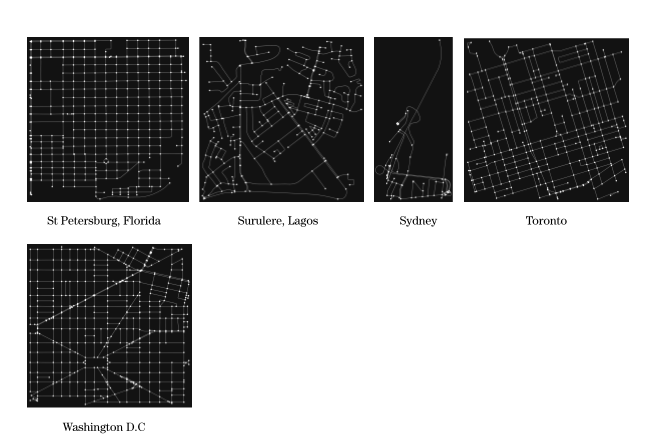
\includegraphics[width=1.0\textwidth,center]{picture/Graphs2.png}
\caption[Miniaturtrichter]{Road Network Graphs}
\label{fig:roadnetworkgraphs}
\end{figure}

\section{Road Network Similarity Metrics}
All the network-similarity metrics used for this study are categorized based on two criteria. First, at what level of the network does the method operate? Second, what type of comparison does it use? For the first criteria 3 levels are defined, they are micro, mezzo, and macro. As their names imply, at the micro-level, a metric extracts features at the node level;1 at the mezzo-level, the metric extracts features from communities; and at the macro-level, it extracts features from the global/network level.  For the second criteria, there are 3 types: vector-based, classifier-based, and matching-based. For this study, we will be using the vector-based and classifier-based types, which are described below. For the Vector-based metrics, feature vectors F1 and F2 are assigned to each network G1 and G2, respectively. They define the similarity between G1 and G2 as 1 − Canberra(F1, F2) [13].2 For the Classifier-based metric,  a fixed number of structures is first identified within each network (such as random walks, communities, or node neighborhoods). For each of these structures, a feature vector is calculated describing its structural properties (e.g., the number of edges within a node neighborhood); and the feature vectors are thereby labeled with the name of their respective network. Cross-validation is then used afterward to determine whether an SVM can accurately distinguish between the feature vectors from network G1 and the feature vectors from network G2. In each round of cross-validation, the test set contains feature vectors from G1 and G2; and so for each of G1 and G2, they create a length-2 feature vector (respectively, F1 and F2) describing the fraction of feature vectors from that network that were classified as belonging to G1 and the fraction that were classified as belonging to G2. They define the similarity between G1 and G2 as 1−Canberra(F1, F2). If G1 and G2 have very similar local structures, then we expect that SVM will not be able to distinguish between the two classes of feature vectors, and F1 and F2 will be very similar. The distance between F1 and F2 will be very low, and so the similarity will be high. Conversely, if G1 and G2 have very different structures, then the SVM will have high classification accuracy and a low similarity score. For the matching-based metric, see () which goes into detail how this approach is described and can be applied. Table 2 categorizes all road network-similarity metrics
based on the two criteria mentioned above. Each of these 10 metrics is briefly described below. Based on previous studies and research (), because macro-level metrics consider the entire network at once, rather than local sub-structures, it is not possible for such metrics to be classifier- or matching-based.

\begin{table}[]
\centering
\resizebox{\textwidth}{!}{%
\begin{tabular}{|l|c|c|c|}
\hline
\multicolumn{1}{|c|}{\textbf{}} &
  \textbf{Micro-Level} &
  \textbf{Mezzo-level} &
  \textbf{Macro-level} \\ \hline
\textbf{Vector Based} &
  NetSimile[], Euclidean Distance [], Cosine Similarity [] &
  Random Walk[] &
  Degree Divergence [], NetLSD[], Laplacian Spectra [] \\ \hline
\textbf{Classifier Based} &
  Jaccard Similarity [] &
  Shortest Path Kernel [], Jaccard Distance [] &
  - \\ \hline
\end{tabular}%
}
\caption{}
\label{tab:Road network similarity metrics used in this study, organized by (1) network level and (2) comparison type.}
\end{table}

\subsection{Shortest Path Kernel}

According to [Karsten M. Borgwardt and Hans-Peter Kriegel. Shortest-path kernels on graphs. In Proceedings of the 5th International Conference on Data Mining, 74–81. 2005.], the shortest-path kernel decomposes graphs into shortest paths and compares pairs of shortest paths according to their lengths and the labels of their endpoints. The first step of the shortest-path kernel is to transform the input graphs into shortest-paths graphs. Given an input graph , a new graph  (i.e. its shortest-path graph) is created. The shortest-path graph  contains the same set of vertices as the graph from which it originates. The edge set of the former is a superset of that of the latter, since in the shortest-path graph , there exists an edge between all vertices which are connected by a walk in the original graph . To complete the transformation, labels are assigned to all the edges of the shortest-path graph . The label of each edge is set equal to the shortest distance between its endpoints in the original graph .

Given the above procedure for transforming a graph into a shortest-path graph, the shortest-path kernel is defined as follows.

Let Gi, Gj be two graphs, with Si, Sj be their corresponding shortest-path graphs.

The shortest-path kernel is then defined on Si  = (Vi, Ei) and Si = (Vj, Ej) as

$$
k\left(S_{i}, S_{j}\right)=\sum_{e_{i} \in E_{i}} \sum_{e_{j} \in E_{j}} k_{w a l k}^{(1)}\left(e_{i}, e_{j}\right)
$$

where $k_{w a l k}^{(1)}\left(e_{i}, e_{j}\right)$ is a positive semidefinite kernel on edge walks of length $1 .$

In labeled graphs, the $k_{\text {walk }}^{(1)}\left(e_{i}, e_{j}\right)$ kernel is designed to compare both the lengths of the shortest paths corresponding to edges $e_{i}$ and $e_{j}$, and the labels of their endpoint vertices.

Let $e_{i}=\left\{v_{i}, u_{i}\right\}$ and $e_{j}=\left\{v_{j}, u_{j}\right\}$. Then, $k_{\text {walk }}^{(1)}\left(e_{i}, e_{j}\right)$ is usually defined as:

$$
\begin{aligned}
k_{\text {walk }}^{(1)}\left(e_{i}, e_{j}\right) &=k_{v}\left(\ell\left(v_{i}\right), \ell\left(v_{j}\right)\right) k_{e}\left(\ell\left(e_{i}\right), \ell\left(e_{j}\right)\right) k_{v}\left(\ell\left(u_{i}\right), \ell\left(u_{j}\right)\right) \\
&+k_{v}\left(\ell\left(v_{i}\right), \ell\left(u_{j}\right)\right) k_{e}\left(\ell\left(e_{i}\right), \ell\left(e_{j}\right)\right) k_{v}\left(\ell\left(u_{i}\right), \ell\left(v_{j}\right)\right)
\end{aligned}
$$

where $k_{v}$ is a kernel comparing vertex labels, and $k_{e}$ a kernel comparing shortest path lengths. Vertex labels are usually compared via a dirac kernel, while shortest path lengths may also be compared via a dirac kernel or, more rarely, via a brownian bridge kernel [BК05].

In terms of runtime complexity, the shortest-path kernel is very expensive since its computation takes $\mathcal{O}\left(n^{4}\right)$ time.

\subsection{Random Walk Kernel}
The most well-studied family of graph kernels is probably the random walk kernels which quantify the similarity between a pair of graphs based on the number of common walks in the two graphs [KTI03], [GartnerFW03], [MaheUA+04], [BOSchonauer+05], [VSKB10], [SB15].

Kernels belonging to this family have concentrated mainly on counting matching walks in the two input graphs. There are several variations of random walk kernels. The -step random walk kernel compares random walks up to length  in the two graphs. The most widely-used kernel from this family is the geometric random walk kernel [GartnerFW03] which compares walks up to infinity assigning a weight  () to walks of length  in order to ensure convergence of the corresponding geometric series. We next give the formal definition of the geometric random walk kernel. Given two node-labeled graphs  and  , their direct product is a graph with vertex set:

assigning a weight $\lambda^{k}(\lambda<1)$ to walks of length $k$ in order to ensure convergence of the corresponding geometric series. We next give the formal definition of the geometric random walk kernel. Given two node-labeled graphs $G_{i}=\left(V_{i}, E_{i}\right)$ and $G_{j}=\left(V_{j}, E_{j}\right)$, their direct product $\boldsymbol{G}_{\times}=\left(V_{\times}, \boldsymbol{E}_{\times}\right)$is a graph with vertex set:

$$
V_{\times}=\left\{\left(v_{i}, v_{j}\right): v_{i} \in V_{i} \wedge v_{j} \in V_{j} \wedge \ell\left(v_{i}\right)=\ell\left(v_{j}\right)\right\}
$$

and edge set:

$$
E_{\times}=\left\{\left\{\left(v_{i}, v_{j}\right),\left(u_{i}, u_{j}\right)\right\}:\left\{v_{i}, u_{i}\right\} \in E_{i} \wedge\left\{v_{j}, u_{j}\right\} \in E_{j}\right\}
$$

Performing a random walk on $G_{\times}$is equivalent to performing a simultaneous random walk on $G_{i}$ and $G_{j}$. The geometric random walk kernel counts common walks (of potentially infinite length) in two graphs and is defined as follows.

{Definition: Geometric Random Walk Kernel}

Let $G_{i}$ and $G_{j}$ be two graphs, let $A_{\times}$denote the adjacency matrix of their product graph $G_{\times}$, and let $V_{\times}$denote the vertex set of the product graph $G_{\times}$.

Then, the geometric random walk kernel is defined as

$$
K_{\times}^{\infty}\left(G_{i}, G_{j}\right)=\sum_{p, q=1}^{\left|V_{\times}\right|}\left[\sum_{l=0}^{\infty} \lambda^{l} A_{\times}^{l}\right]_{p q}=e^{T}\left(I-\lambda A_{\times}\right)^{-1} e
$$

where $I$ is the identity matrix, $e$ is the all-ones vector, and $\lambda$ is a positive, real-valued weight. The geometric random walk kernel converges only if $\lambda<\frac{1}{\lambda_{\times}}$where $\lambda_{\times}$is the largest eigenvalue of $A_{\times}$.

Direct computation of the geometric random walk kernel requires $\mathcal{O}\left(n^{6}\right)$ time. The computational complexity of the method severely limits its applicability to real-world applications. To account for this, Vishwanathan et al. proposed in [VSKB10] four efficient methods to compute random walk graph kernels which generally reduce the computational complexity from $\mathcal{O}\left(n^{6}\right)$ to $\mathcal{O}\left(n^{3}\right)$. Mahé et al. proposed in [MaheUA+04] some other extensions of random walk kernels. Specifically, they proposed a label enrichment approach which increases specificity and in most cases also reduces computational complexity. They also employed a second order Markov random walk to deal with the problem of "tottering". Sugiyama and Borgwardt focused in [SB15] on a different problem of random walk kernels, a phenomenon referred to as "halting".


\subsection{NetLSD}
The NetLSD distance LSD between two graphs, $G$ and $G^{\prime}$, is the Frobenius norm between the heat trace signatures of the normalized Laplacians $\mathbf{L}$ and $\mathbf{L}^{\prime}[3]$. The heat kernel matrix is calculated as

$$
H_{t}=e^{-t \mathbf{L}}=\sum_{j=1}^{n} e^{-t \lambda_{j}} \phi_{j} \phi_{j}^{T}
$$

The $i j$-th element of $H_{t}$ contains the amount of heat transferred from node $v_{i}$ to node $v_{j}$ at time $t$ (default of 256 log-spaced time intervals between $10^{-2}$ and $10^{2}$ ). From the heat kernel matrix $H_{t}$, the heat trace, $h_{t}$ is defined as

$$
h_{t}=\operatorname{Tr}\left(H_{t}\right)=\sum_{j=1}^{n} e^{-t \lambda_{f}}
$$

The heat trace signature of graph $G$ is the set $\left\{h_{t}\right\}_{t \geq 1}$. Upon computing heat trace signatures of both $G$ and $\bar{G}^{\prime}$, they are compared via a Frobenius norm

$$
D_{\mathrm{LSD}}\left(G, G^{\prime}\right)=d_{\mathrm{FRO}}\left(\left\{h_{t}\right\}_{t \geq 0},\left\{h_{t}^{\prime}\right\}_{t \geq 0}\right) .
$$

The computational complexity of LSD is $O\left(n^{3}\right)$ due to the spectral decomposition of the Laplacian matrices of both graphs (see Appendix B 4).

\subsection{Degree Divergence}
A simple graph distance measure is the JensenShannon divergence [54] between the empirical degree distributions of two graphs. In this case for an $n$-node graph $G$ the descriptor $\psi_{G}$ is the empirical degree distribution encoded in the set of numbers $\left\{p_{k}(G)\right\}_{k \geq 0}:=\mathbf{p}$ given by $p_{k}(G):=n_{k}(G) / n$, where $n_{k}(G)=\sum_{i=1}^{n} 1\left\{k_{i}=\right.$ $k\}$, with $1\{-\}$ being the indicator function and $k_{i}=$ $\sum_{j=1}^{n} A_{i j}$ being the degree of node $i$ in terms of the adjacency matrix A of $G$. The Jensen-Shannon divergence between two such distributions $[34]$ is the degree JensenShannon divergence or DJS distance between the graphs:

$$
D_{\text {DJs }}\left(G, G^{\prime}\right)=H\left[\mathbf{p}_{+}\right]-\frac{1}{2}\left(H[\mathbf{p}]+H\left[\mathbf{p}^{\prime}\right]\right)
$$

where $\mathbf{P}_{+}=\left\{\left(p_{k}+p_{k}^{\prime}\right) / 2\right\}_{k \geq 0}$ is a mixture distribution and $H[\mathbf{p}]=-\sum_{k} p_{k} \ln p_{k}$ is the Shannon entropy. The computational complexity of DJS is $O(n)$, which arises from computing two degree distributions (which is $O(n)$ ) and then comparing them (which is $O\left(k_{+}\right)$, with $k_{+}<n$ being the maximum degree in either network).

\subsection{Laplacian Spectra}
the methods below, we use the eigenvalues $\left\{\lambda_{1}=0 \leq\right.$ $\left.\lambda_{2} \leq \cdots \leq \lambda_{n}\right\}$ of the normalized Laplacian matrices $\mathbf{L}$ and $\mathbf{L}^{\prime}$. To perform the comparison, a subset of the whole spectrum can be used, e.g. the $k$ smallest [61] or largest $[6,27]$ in magnitude. Unless specified, we used all eigenvalues for comparison $(k=n)$.

The distances compare the continuous spectra $\rho(\lambda)$ and $\rho^{\prime}(\lambda)$ associated with the graph $G$ and $G^{\prime}$. A continuous spectrum is obtained by the convolution of the discrete spectrum $\sum_{i} \delta\left(\lambda-\lambda_{i}\right)$ with a kernel $g\left(\lambda, \lambda^{*}\right)$

$$
\rho(\lambda)=\frac{1}{Z} \sum_{i=1}^{n} \int_{0}^{2} g\left(\lambda, \lambda^{*}\right) \delta\left(\lambda^{*}-\lambda_{i}\right) \mathrm{d} \lambda^{*},
$$

where $Z$ is a normalization factor. Different types of distribution can be used for the kernel, for instance a Lorentzian distribution [43]

$$
g\left(\lambda, \lambda^{*}\right)=\frac{\gamma}{\pi\left[\gamma^{2}+\left(\lambda-\lambda^{*}\right)^{2}\right]},
$$

or a Normal distribution

$$
g\left(\lambda, \lambda^{*}\right)=\frac{\exp \left[-\left(\lambda-\lambda^{*}\right)^{2} / 2 \sigma^{2}\right]}{\sqrt{2 \pi \sigma^{2}}} .
$$

Different types of metrics can then be used to compare the spectra, such as the Euclidean metric

$$
d\left(\rho, \rho^{\prime}\right)=\sqrt{\int_{0}^{2}\left[\rho(\lambda)-\rho^{\prime}(\lambda)\right]^{2} \mathrm{~d} \lambda},
$$

or the square root of the $\operatorname{JSD} d\left(\rho, \rho^{\prime}\right)=\sqrt{J S D\left(\rho, \rho^{\prime}\right)}$, written as

$$
J S D\left(\rho, \rho^{\prime}\right)=\frac{1}{2} D_{K L}(\rho \| \bar{\rho})+\frac{1}{2} D_{K L}\left(\rho^{\prime} \| \bar{\rho}\right)
$$

where $\bar{\rho}=\left(\rho+\rho^{\prime}\right) / 2$. Various combination of kernels and metrics yield the following distinct distance measures:

- Laplacian spectrum: Gaussian kernel, JSD distance LGJ

- Laplacian spectrum: Lorenzian kernel, Euclidean distance LLE

For both kernels, we use a half width at half maximum of $0.011775$ (which means the standard deviation for the Gaussian kernel is $\approx 0.01$ ).

While we only focus on the two specific distances above, we note again that there is a world of possible combinations of descriptor-distance pairs to possibly use for comparing graphs. We selected the two above because their within-ensemble graph distance curves differed the most (e.g. as opposed to including Gaussian kernel / Euclidean distance or Lorenzian kernel / JSD). The computational complexity of this suite of graph distances is $O\left(n^{3}\right)$ due to the spectral decomposition of the Laplacian matrices of both graphs (see Appendix B 4).

\subsection{NetSimile}
NetSimile NES is a method for comparing two graphs, $G$ and $G^{\prime}$, that is based on statistical features of the two graphs. It is invariant to graph labels and is able to compare graphs of different sizes [1]. It is calculated as the Canberera distance between the $7 \times 5$ feature matrix, $\mathbf{p}$ and $\mathbf{p}^{\prime}$, of each graph. To construct the $\mathbf{p}$ and $\mathbf{p}^{\prime}$ feature matrices, first a $7 \times n$ matrix is constructed for each, with each column, $j$, consisting of the following seven node-level quantities:

1. degree, $k_{j}=\sum_{j} A_{i j}$

2. clustering coefficient, $c_{j}=\left(A^{3}\right)_{j j} /\left(\begin{array}{c}k_{j} \\ 2\end{array}\right)$

3. average neighbor degree $k_{j}^{(n n)}=\frac{1}{k_{j}} \sum_{i} k_{i} A_{i j}$.

4. average clustering coefficient of the nodes in the ego network $c_{j}^{(e g o)}=\sum_{i} c_{i} A_{i j}$

5. number of edges within the ego network $T_{j}=$ $\sum_{l, m} A_{j l} A_{l m} A_{m j}$

6. number of outgoing edges from the ego network $O_{j}=\sum_{i} A_{i j} k_{i}-T_{j}=k_{j} k_{j}^{(n n)}-T_{j}$

7. number of neighbors of the ego network $n n_{j}^{(e g o)}=$ $\sum_{i} 1_{\left\{\exists l \in \mathcal{N}_{f}: i \sim l, i \chi_{j}\right\}}$

These features are then summarized into $\mathbf{p}$ and $\mathbf{p}^{\prime}$, which are $7 \times 5$ signature vectors consisting of the median,mean, standard deviation, skewness, and kurtosis of each feature. NetSimile uses the Canberra distance to arrive at a final scalar distance.

$$
D_{\mathrm{KSE}}\left(G, G^{\prime}\right)=d\left(\mathbf{p}, \mathbf{p}^{\prime}\right)=\sum_{i=1}^{n} \frac{\left|p_{i}-p_{i}^{\prime}\right|}{\left|p_{i}\right|+\left|p_{i}^{\prime}\right|}
$$

The computational complexity of NES depends on two parts : features extraction and features aggregation. Features are all locally defined, hence their extraction will take $O(q n)$ where $q$ is the average degree of a node when selecting a random edge and choosing an endpoint [63]. Feature aggregation is $O(n \ln n)[1]$, hence the overall complexity is $O(q n+n \log n)$.

\subsection{Cosine Similarity}
Originally used in text mining for document comparison, the cosine similarity computes the angle between the document vectors, without taking into account their lengths. It assigns higher similarity to vectors that point roughly in the same direction. 
Returns: the cosine similarity values in [-1, 1]. the cosine similarity values are converted to a similarity measure in the range [0, 1]. According to literature, the most prevalent ways of deriving the similarity measure are the following:

According to literature, the most prevalent ways of deriving the similarity measure are the following: 
- $s=1-d$
- $s=\frac{1}{d}$
- $s=\frac{1}{1+d}$ for unbounded $d$
$s=e^{-d^{2}}$

\subsection{Euclidean Distance}
Based on the Euclidean distance measurement approach, the euclidean based similarity  is a normalized euclidean similarity measure that calculates the shortest distance between 2 points irrespective of their dimensions.  Returns: the calculated distance (d) converted to a similarity measure (s) in the range [0, 1].

Compute the distance matrix between each pair from a vector array $\mathrm{X}$ and $\mathrm{Y}$.
For efficiency reasons, the euclidean distance between a pair of row vector $x$ and $y$ is computed as:
$\operatorname{dist}(x, y)=\operatorname{sqrt}(\operatorname{dot}(x, x)-2 * \operatorname{dot}(x, y)+\operatorname{dot}(y, y))$
This formulation has two advantages over other ways of computing distances. First, it is computationally efficient when dealing with sparse data. Second, if one argument varies but the other remains unchanged, then dot ( $x, x)$ and/or dot ( $y$, $y$ ) can be pre-computed.
However, this is not the most precise way of doing this computation, because this equation potentially suffers from "catastrophic cancellation". Also, the distance matrix returned by this function may not be exactly symmetric as required by, e.g., scipy. spatial. distance functions.
Read more in the User Guide. An array where each row is a sample and each column is a feature.
Y : \{array-like, sparse matrix $\}$ of shape (n_samples_ $Y, n_{-}$features), default=None An array where each row is a sample and each column is a feature. If None, method uses $Y=X$. default=None
Pre-computed dot-products of vectors in $Y$ (e.g., $(Y * * 2) .$ sum (axis=1)) May be ignored in some cases, see the note below.
squared : bool, default=False
Return squared Euclidean distances.
Pre-computed dot-products of vectors in $X($ e.g., $(X * * 2)$. sum(axis=1)) May be ignored in some cases, see the note below.
Returns: distances : ndarray of shape (n_samples_X, n_samples_Y) Returns the distances between the row vectors of $X$ and the row vectors of $Y$.

\subsection{Jaccard Similarity}

\subsection{Jaccard Distance}
The Jaccard measure is computed using the adjacency matrix $\psi_{G}=\mathbf{A} \in\{0,1\}^{n \times n}$. For two graphs vertexlabeled $G$ and $G^{\prime}$,

$$
D_{\mathrm{JAC}}\left(G, G^{\prime}\right)=d_{\mathrm{JAC}}\left(\mathbf{A}, \mathbf{A}^{\prime}\right)=1-\frac{|\mathbf{S}|}{|\mathbf{T}|}
$$

where $S_{i j}=A_{i j} A_{i j}^{\prime}$ represents the intersection of edge sets between graphs $G$ and $G^{\prime}$, while $T_{i j}=S_{i j}+(1-$ $\left.A_{i j}^{\prime}\right) A_{i j}+\left(1-A_{i j}\right) A_{i j}^{\prime}$ represents the union of edge sets between graphs. Here, $|\mathbf{S}|$ is the sum over the $S_{i j}$ and similarly for $|\mathbf{T}|$. The computational complexity of the Jaccard distance is $O\left(|E|+\left|E^{\prime}\right|\right)$ when using unordered sets to get the union and intersection sets and their cardinality. This is what is done in the netrd package [51]. Since nearly empty graphs likely have nearly zero edges in common, the $|\mathbf{S}||\mathbf{T}|$ will be nearly zero for $p$ close to 0 , so that $d_{J A C}$ approaches 1 at low $p$.

